\documentclass[fleqn,a4paper,12pt]{article}
\usepackage{standalone}		% Zum Einlesen aus anderen .tex-Files
\usepackage{geometry}		% Zur Bearbeitung des Layouts (Ränder,...)
\geometry{left=30mm, right=40mm, bottom=30mm}
\usepackage[german]{babel}
\usepackage[utf8]{inputenc}
\usepackage{amsmath}		% Mathematische Symbole
\usepackage{amssymb}     	% Nochmehr mathematische Symbole
\usepackage{dsfont}      	% Schriftsatz fuer Zahlenmengensymbole
%\usepackage{verbatim}   	% erweiterte Verbatim-Umgebung
\usepackage{alltt}       	% Quasi-Verbatim-Umgebung
\usepackage{fancyhdr}    	% Eigene Kopfzeilen
\usepackage{graphicx}    	% Zum Einbinden von Grafiken
% Einbinden einer eps-Grafik geht so: includegraphics{path}
\usepackage{wrapfig}
\usepackage{lscape}
\usepackage{rotating}
\usepackage{epstopdf}

% Skalierung der Grafiken
\setlength{\unitlength}{1cm}

\pagestyle{fancy}            % Eigene Kopfzeilen verwenden
\frenchspacing               % Kein Extrafreiraum nach Satzzeichen
\setlength{\parindent}{0pt}  % Neue Absaetze nicht einruecken
%\sloppy                     % Schlampige Absatzformatierung
\fussy                       % Penible Absatzformatierung
\linespread{1.5}             % Zeilenabstand

%andere Definitionen
\newcommand{\R}{{\mathbb R}}
\newcommand{\N}{{\mathbb N}}
\newcommand{\Z}{{\mathbb Z}}
\newcommand{\Q}{{\mathbb Q}}
\newcommand{\C}{{\mathbb C}}
\newcommand{\F}{\mathcal{F}}
\newcommand{\less}{\setminus}
\newcommand{\inv}{{}^{-1}}
\newcommand{\Land}{\bigwedge}
\newcommand{\Lor}{\bigvee}

\begin{document}
	"Ubungsaufgabe 8: \newline
	Sei folgendes Tertiärsignal gegeben:\\
	\begin{tabular}{|c|p{0.6cm}|p{0.35cm}|p{0.35cm}|p{0.35cm}|p{0.35cm}|p{0.35cm}|p{0.35cm}|p{0.35cm}|p{0.35cm}|p{0.35cm}|p{0.5cm}|p{0.15cm}|p{0.2cm}|p{0.2cm}|p{0.2cm}|p{0.2cm}|p{0.2cm}|p{0.2cm}|p{0.2cm}|p{0.2cm}|p{0.4cm}|}
		\hline
		Messwert	& -10 & -9 & -8 & -7 & -6 & -5 & -4 & -3 & -2 & -1 & 0 & 1 & 2 & 3 & 4 & 5 & 6 & 7 & 8 & 9 & 10\\
		\hline
		Anzahl		& 1 & 2 & 3 & 4 & 50 & 6 & 5 & 4 & 3 & 2 & 228 & 2 & 3 & 4 & 5 & 6 & 50 & 4 & 3 & 2 & 1\\
		\hline
	\end{tabular}\\
	\\
	Aus den 388 Daten der Zufallsvariable $X$ lassen sich nun folgende Werte entnehmen:
	\begin{align*}
	m_1 = E[X]				=& \int_\Z x\rho(x) \mu(dx) = \sum_{x=-10}^{10} x\rho(x)= \frac{0}{388} = 0\\
	z_2 = Var(X) = \sigma^2	=& E\left[\left(X-E[X]\right)^2\right] = E\left[X^2 - 2E[X]X + E[X]^2\right]\\
	=& E\left[X^2\right] - E\left[2E[X]X\right] + E\left[E[X]^2\right]\\
	=& E\left[X^2\right] - 2E[X]E\left[X\right] + E[X]^2 E\left[1\right]\\
	=& E\left[X^2\right] - 2E[X]^2 + E[X]^2 \cdot 1 = E\left[X^2\right] - E[X]^2\\
	=& \int_\Z x^2\rho(x) \mu(dx) - E[X]^2 = \sum_{x=-10}^{10} x^2\rho(x) - 0^2\\
	=& \frac{5460}{388} \approx 14,07\\
	\sqrt{z_2} = \sigma		\approx& 3,75\\
	\end{align*}
	Wobei, wie aus Stochastik I bekannt, der Erwartungswert von $X$ $E[X]$ ein lineares Funktional, $\mu$ das kanonische Zählmaß und $\rho(x)$ die relative Häufigkeit von $x$ ist\\
	\\
	Da $m_1 = E[X] = 0$ gilt $\forall i\in\N:m_i = z_i$\\
	$z_0 = \sum_{x=-10}^{10} \rho(x) = 1$ nach Definition.\\
	$z_1 = m_1 = 0$\\
	$z_2 \approx 14,07$\\
	$z_3 = \sum_{x=-10}^{10} x^3\rho(x) =  0$\\
	$z_4 = \sum_{x=-10}^{10} x^4\rho(x) \approx  593,91$\\
	\newpage
	\begin{figure}
		%\centering
		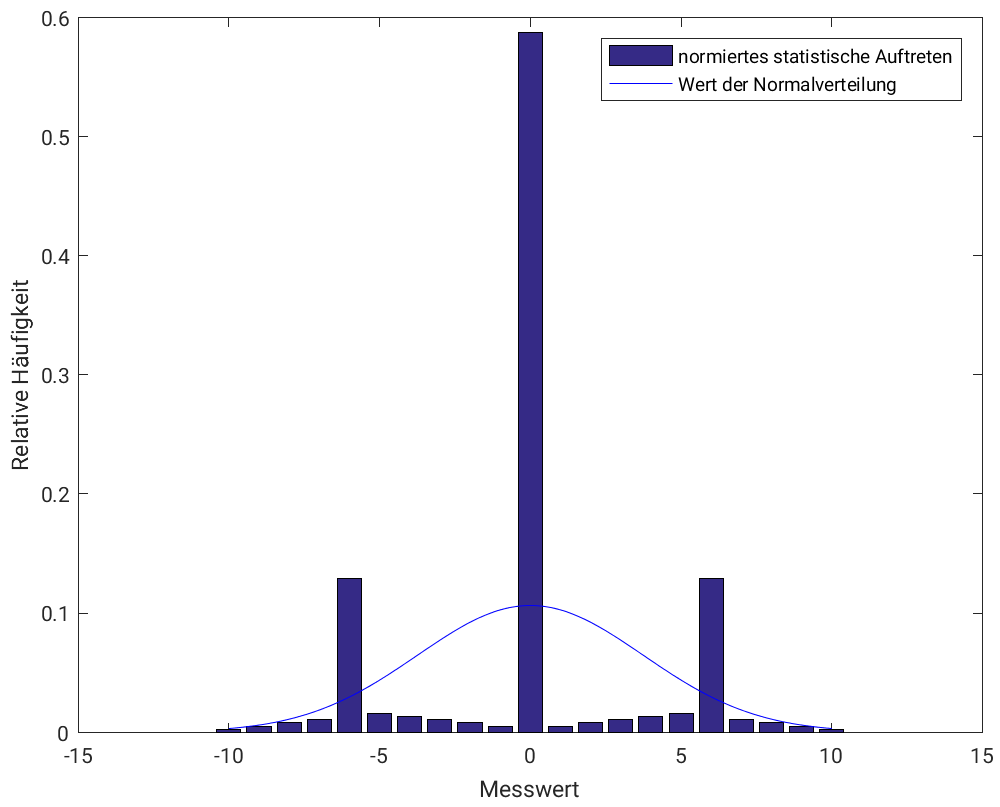
\includegraphics[scale = 0.9]{A08_Histogramm.png}
		\caption{Darstellung des Histogramms und der Glockenkurve}
	\end{figure}
	Mit der Formel $\mathfrak{Z}_k := \frac{z_k}{\sqrt{z_2^k}}$ ergibt sich:\\
	$\mathfrak{Z}_0 := \frac{z_0}{\sqrt{z_2^0}} = \frac{1}{1} = 1$\\
	$\mathfrak{Z}_1 := \frac{z_1}{\sqrt{z_2^1}} = \frac{0}{\sigma} = 0$\\
	$\mathfrak{Z}_2 := \frac{z_2}{\sqrt{z_2^2}} = \frac{z_2}{z_2} = 1$\\
	$\mathfrak{Z}_3 := \frac{z_3}{\sqrt{z_2^3}} = \frac{0}{\sqrt{z_2^3}} = 0$\\
	$\mathfrak{Z}_4 := \frac{z_4}{\sqrt{z_2^4}} = \frac{z_4}{z_2^2} \approx \frac{593,91}{197,96} \approx 3,0$\\
	\\
	Nach den normierten Zentralmomenten hat das gegebene Ternärsignal die selbe Symmetrie und Wölbung wie die Glockenkurve.	
\end{document}